\section{Tổng quan}
\subsection{Ngôn ngữ lập trình sử dụng: Python}
\subsection{Môi trường hệ điều hành: Windows}

\section{Mô tả chương trình}
\subsection{Chạy phía server}
\subsection{Chạy phía client}
\bf
\begin{enumerate}
\large\item Giao diện
\normalsize
\begin{figure}[H]
\center{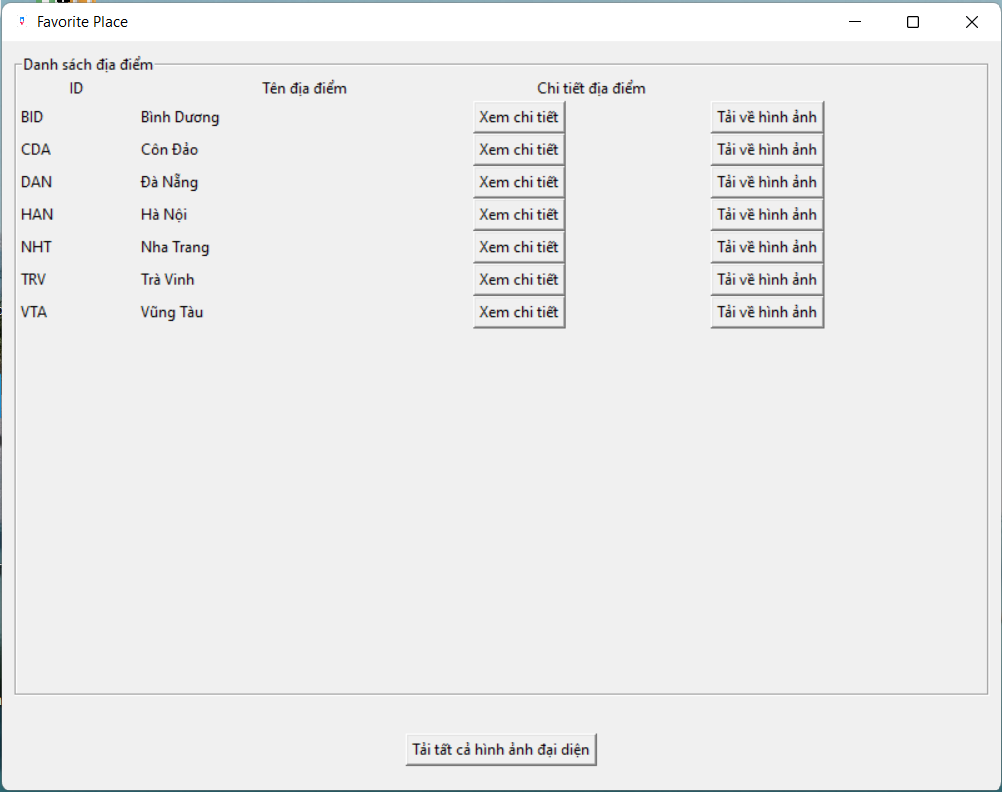
\includegraphics[scale=0.75]{app-description/app}}
\caption{Giao diện phần mềm phía \texttt{client}}
\end{figure}

\large\item \bf Tính năng
\normalsize
\begin{enumerate}
\item \textit{Truy vấn chi tiết thông tin địa điểm}


\item \textit{Tải về tất cả hình ảnh của địa điểm}
\end{enumerate}
\end{enumerate}

